\begin{blocksection}
\question Draw the environment diagram that results from running the code below.

\begin{lstlisting}
def reverse(lst):
    if len(lst) <= 1:
        return lst
    return reverse(lst[1:]) + [lst[0]]

lst = [1, [2, 3], 4]
rev = reverse(lst)
\end{lstlisting}

\begin{solution}[2in]
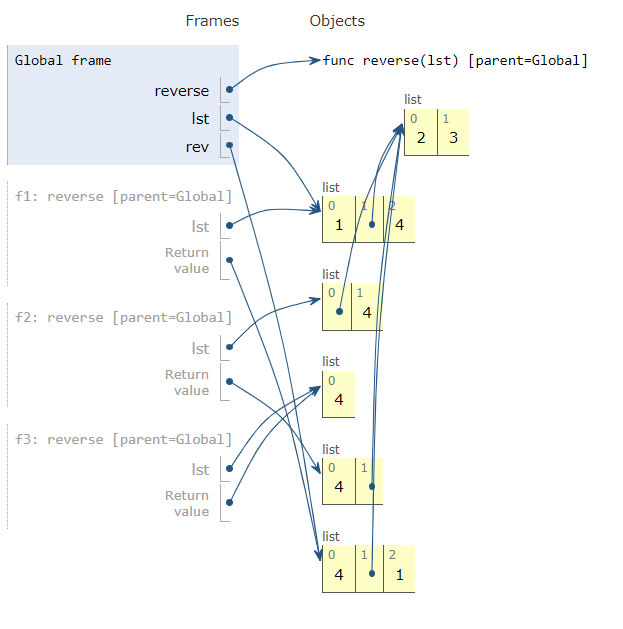
\includegraphics[width=0.7\textwidth]{reverse.png}

\url{https://goo.gl/6vPeX9}
\end{solution}
\end{blocksection}

\begin{questionmeta}
\textbf{Teaching Tips}
\begin{itemize}
    \item We call \lstinline{reverse} recursively 3 times and open 3 new frames, each time passing through a shallow copy of the list without the first element
    \item We then return the list \lstinline{[4]} after hitting the base case of a length 1 list.
    \item At each level, we take the list returned from the smaller recursive call and append \lstinline{lst[0]} to the end of returned list.
    \item When you pass in a list as an argument to a function, the new frame’s argument points to the same list passed in (it does not create a new list!)
    \item List slices create shallow copies (a new list is created but any pointers in the new list still point to the same thing)
    \item Keep in mind that the return value of the reverse function is a new list because of the \lstinline{+ [lst[0]]}
\end{itemize}
\end{questionmeta}
